\documentclass[a4paper]{article}
\usepackage[utf8]{inputenc}
\usepackage{float}
\usepackage{pdfpages}
\usepackage{textcomp}
\usepackage{indentfirst}

\setlength{\parskip}{1em}

% Colour Management
\usepackage{color}

% Multi-Line Comments
\usepackage{comment}

% Customisable Sections
\usepackage{titlesec}

% Images and Captions
\usepackage{graphicx}
\usepackage{subcaption}
\usepackage{wrapfig}
\graphicspath{{./images/}}
\usepackage{fancyhdr} 


% Bibliography
\usepackage[nottoc]{tocbibind}
\usepackage[
    backend=biber,
    style=ieee]{biblatex}

\addbibresource{report_citations.bib} %Imports bibliography file



% Tables
\usepackage{xcolor}
\usepackage{array}
\newcolumntype{L}{>{\raggedright\arraybackslash}m{0.9\linewidth}}

% Contents Page
\usepackage{hyperref}

% Appendices
\usepackage[toc,page]{appendix}

% Bold Maths Symbols
\usepackage{bm}
\usepackage{amsmath} %sudo tlmgr install amsmath
\usepackage{gensymb} %sudo tlmgr install was
\usepackage{multicol}

%Command for adding units to equations
\newcommand{\unit}[1]{\ensuremath{\, \mathrm{#1}}}


% Allowing lower levels of Contents Page
\setcounter{tocdepth}{4}
\setcounter{secnumdepth}{5}

% Make margins smaller, feel free to change
\usepackage{geometry}
\geometry{
    a4paper,
    top = 20mm,
    bottom = 20mm,
    textwidth=426pt
}





\title{Engineering Design Project}
\author{Georgio Chaimali \and 
        Dimitrios Georgakopoulos \and 
        Edvard J. Skaarberg Holen \and 
        Hyunjoon Jeon \and 
        Josiah Mendes \and 
        Raghav Viswakumar}
\begin{document} 
\begin{titlepage}
    \setlength{\headheight}{66.89pt}
    \thispagestyle{fancy}
    \renewcommand{\headrulewidth}{0pt}
    \renewcommand{\footrulewidth}{0pt}
    \lhead{
\includegraphics[scale=0.1]{logo.png}}
    \cfoot{} % this is to remove the page number
    \hbox{}\vfill
    \begin{center} 
	    {\scshape\LARGE Imperial College London  \par}
	    \vspace{1cm}
        {\scshape\Large Second Year Design Project\par}
        \vspace{0.25cm}
        {\scshape\Large ELEC50003/ELEC50008\par}
        \vspace{1.5cm}
        {\huge\bfseries The MARS Rover\par}
        \vspace{2cm}
        {\Large\itshape Group 1\par}
        \vfill
        \begin{flushright}
            \textsl{ \large
            Georgio Chaimali \\ 
            Dimitrios Georgakopoulos \\ 
            Edvard J. Skaarberg Holen \\ 
            Hyunjoon Jeon \\ 
            Josiah Mendes \\ 
            Raghav Viswakumar
            }
        \end{flushright}
        \vfill

        % Bottom of the page
        {\large Word Count: XXXX Words \\ \today\par}
    \end{center}
\end{titlepage}
 
\setcounter{tocdepth}{2}
\tableofcontents

\newpage

\section{Overview}

\section{Systems}

\subsection{Control}

\subsubsection{Overview of Module and Goals}
The Control module within the context of the rover has one main goal: 
to act as the communication hub between all the subsystems, delivering
the relevant data where it is required to allow for the rover to integrate
as a whole \cite{MarsRoverSpec}. There are a couple of core objectives which must be 
achieved in order to fulfill this role and they are as follows:

\begin{enumerate}
    \item Act as a Wifi Access Point sitting under a router to receive
    commands from the Command subsystem and send data through socket-level communication.
    \item Use a relevant hardware-level data transmission protocol to
    send movement commands to the Drive subsystem and receive data for Command. 
    \item Use a relevant hardware-level data transmission protocol to receive
    the Vision subsystem data.
    \item Connect the Energy subsystem with the rover, sending the relevant data
    to the Command subsystem.
\end{enumerate}

Although the hardware is fixed, the solutions to the outlined problems
above are mostly up to design. It is for this reason that the main challenge
stems from understanding what works best for communication to each subsystem
and more importantly, how to integrate it such that the transmission of data
can be smoothly facilitated through the ESP32.

\subsubsection{Hardware Organisation}

The Control module comprises of two hardware components \cite{BoxContent}: 
the ESP32, a system on chip microcontroller \cite{ESP32Datasheet}, as well as an Arduino adapter
board designed to map some of the available GPIO pins on the ESP32 to an Arduino-like
board \cite{ESP32ArduinoAdapter}.

This hardware was provided by the project organisers and it immediately limits
the tools which can be used, however the wide array of functionality which
this microcontroller can provide through programming the chip allows
for sufficient freedom and capabilities to complete the required tasks. The
GPIO pins are highly configurable when compared to an Arduino-Uno \cite{MicrocontrollerComparison}, as they
are capable of using more data communication through almost any of the pins
via software configuration \cite{ESP32PinOut}. It is low-cost and low-power, 
capable of using Wifi capabilities at 2.4GHz and Bluetooth \cite{ESP32Datasheet} to interface wirelessly
with other devices. Using the Arduino Adapter board \cite{ESP32ArduinoAdapter}, it can sit directly on top of
an Arduino or device with similar pins to directly interface through physical connections. 


\subsubsection{Drive and Control}

\subsubsection{Vision and Control}

\subsubsection{Command and Control}

\subsection{Comms}

\subsection{Vision}
\begin{abstract}
    The purpose of the Vision module is threefold:
    1. Capture data from camera module;
    2. Detect objects of interest within the current view and 
        send their location to the Control module; and
    3. Send image data to Control for streaming to Command. 
\end{abstract}

\subsubsection{Hardware Organisation}

The Vision module comprises of two main hardware elements: 
    the Terasic DE10-Lite, a cost-effective Intel MAX 10 based FPGA board 
    \cite{TerasicDE10Web} 
    and the Terasic D8M-GPIO camera package \cite{TerasicD8MWeb}
that interfaces with the FPGA through the onboard GPIO connectors. 

These hardware choices were made by the project organisers, 
but are also sufficient and capable of carrying out the tasks at hand. 
As the FPGA's hardware is configurable, 
it is more flexible than other embedded systems 
that are limited to a general purpose processor,and 
is also able to handle both streaming and processing of high resolution images
without significant compromises on framerate or data speed 
through the use of concurrent operations and dedicated blocks 
for signal processing applications like multiplication.
This particular FPGA is also equipped with a 4-bit VGA output 
which is useful for debugging object detection live, 
and also has a connector for an Arduino Uno R3 shield, \cite{TerasicDE10Web} 
which can be used to interface with the ESP32 used for control.  

In order to perform general purpose operations like
    to configure camera settings
    and to provide a debugging interface,
a Nios II soft core was instantiated on the FPGA. 
Alternatively, to implement more advanced image processing algorithms
or to reduce other hardware components in the system like the multiple Arduinos, 
a FPGA with a hard core connected via PCIe, 
known as a FPGA System-On-Chip (FPGA SoC) \cite{FPGASoC} could be used, 
which would provide both the advantages of having reconfigurable hardware,
a more capable general purpose processor and a higher bandwidth limit. 

\subsubsection{Image Capture \& Processing Stream}

The image capture and buffering is based on a starter project provided
by Terasic Inc for the D8M Camera module that was modified by Dr Edward Stott 
\cite{EEE2Rover} and provided to us for this project. The system makes use of 
several IP components from the Intel Video and Image Processing Suite,
namely the Clocked Video Output and Frame Buffer Core. The system is compromised
of several modules, that take the raw data from the camera in Bayer filter form\cite{TerasicD8MWeb},
transform it into RGB video packets, buffer the frames to allow camera and output
to run at different frame rates, process the image data and convert the video 
data to serial data for output over VGA.\cite{EEE2Rover} As this system and its 
corresponding documentation is openly available, the implementation outside of 
the image processor will not be described in more depth, interested readers can 
consult the provided repository and starter project for reference. 

\subsubsection{Design \& Implementation of Image Processing Module}

The challenge for this rover was to detect different coloured ping-pong balls as
obstacles and relay the information about these obstacles to the control module. 
The provided ping-pong balls came in 5 different colours - pink, orange, light 
blue, grey and green. As these colours cover a wide range of the colour spectrum
and even overlap with each other (orange and pink, blue and grey), it was 
necessary to implement an algorithm that could take into account the location 
and shape of the ball, as a purely colour based algorithm would be unable to 
differentiate other objects in view of the camera and confuse them with the ball, 
for example, the sky and the light blue ball would be seen as one object. 
 
%Maybe add Image of all the balls here. 


The initial design and implementation of this image processing algorithm involved
a transform from the RGB (Red, Green, Blue) colour space to the HSV (Hue, 
Saturation, Value) colour space, and pixel based classification to detect large
areas of the necessary colours.  HSV has been shown to be a better colour space
for image processing tasks like colour segmentation in road sign detection for 
autonomous driving as it is invariant to illumination changes unlike the RGB 
space.\cite{ali2013performance} As the task at hand here is similar, a transformation
from the RGB space to the HSV space is applied. 

HSV is traditionally expressed as three values ranging between 0-360\degree\  
for hue, and two values between 0 and 1 for saturation and value.\cite{10.1145/965139.807361}
As floating point calculations in SystemVerilog are computationally expensive, 
and also introduce a layer of unnecessary complexity, the conversion was adjusted
to express all three values in terms of an 8 bit integer ranging from 0-255. The
algorithm for conversion is presented mathematically:

\begin{multicols}{3}
    \noindent
    \begin{align*}
        M &= \max(R, G, B) \\ \\
        m &= \min(R, G, B) \\ \\
        C &= M-m 
    \end{align*}
    \begin{equation*}
        H = \begin{cases}
            M = R, & 0 + \frac{43 \times (G-B)}{C} \\
            M = G, & 85 + \frac{43 \times (B-R)}{C} \\
            M = B, & 171 + \frac{43 \times (R-G)}{C} \\
            M = 0, & 0 \\
            C = 0, & 0
        \end{cases} 
    \end{equation*}
    \begin{align*}
        S &= \begin{cases}
            M = 0, & 0 \\ C = 0, & 0 \\ \text{else} & \frac{255\times C}{V}
        \end{cases} & \\ \\
         V &= M  
    \end{align*}
\end{multicols}



Although the inclusion of a divide operation was undesirable as it does not 
translate well to hardware implementations, it was unavoidable with hue being 
obtained by dividing the difference of two components by the chroma value. This 
module was then implemented using two pipelined 3 cycle divider from the Intel IP
megafunction library for the hue and saturation value calculations.  



\subsection{Drive}

% Start of energy subsection
\subsection{Energy}
\begin{abstract}
The main goal of the energy sub-module is to design a battery pack for the rover and charge it using solar power. With this goal in mind, the energy sub-module must develop a battery management system which allows the tracking of battery SOC and SOH, and if necessary perform SOH maintenance. 
    
\end{abstract}

\subsubsection{Characterising Components}
When designing a system it is necessary to know the behaviour and limitations of its constituent components. There are three main components that make up the energy subsystem: the battery cells, the PV panels and the SMPS.

\textbf{\chapter{Battery Cells}} 
\newline
\newline
To determine the behaviour of the battery cells they were all tracked through a full charge/discharge 
cycle using the provided “Battery\_Charge\_Cycle\_Logged\_V1.1.ino” code\cite{chargeCode}. 
Every cell behaved similarly in terms of the cell voltage compared to time. 
The cell voltage of cell 1 over a full discharge/charge cycle is shown in Figure~\ref{fig:charge_cycle}:

\begin{figure}[H]
    \centering
    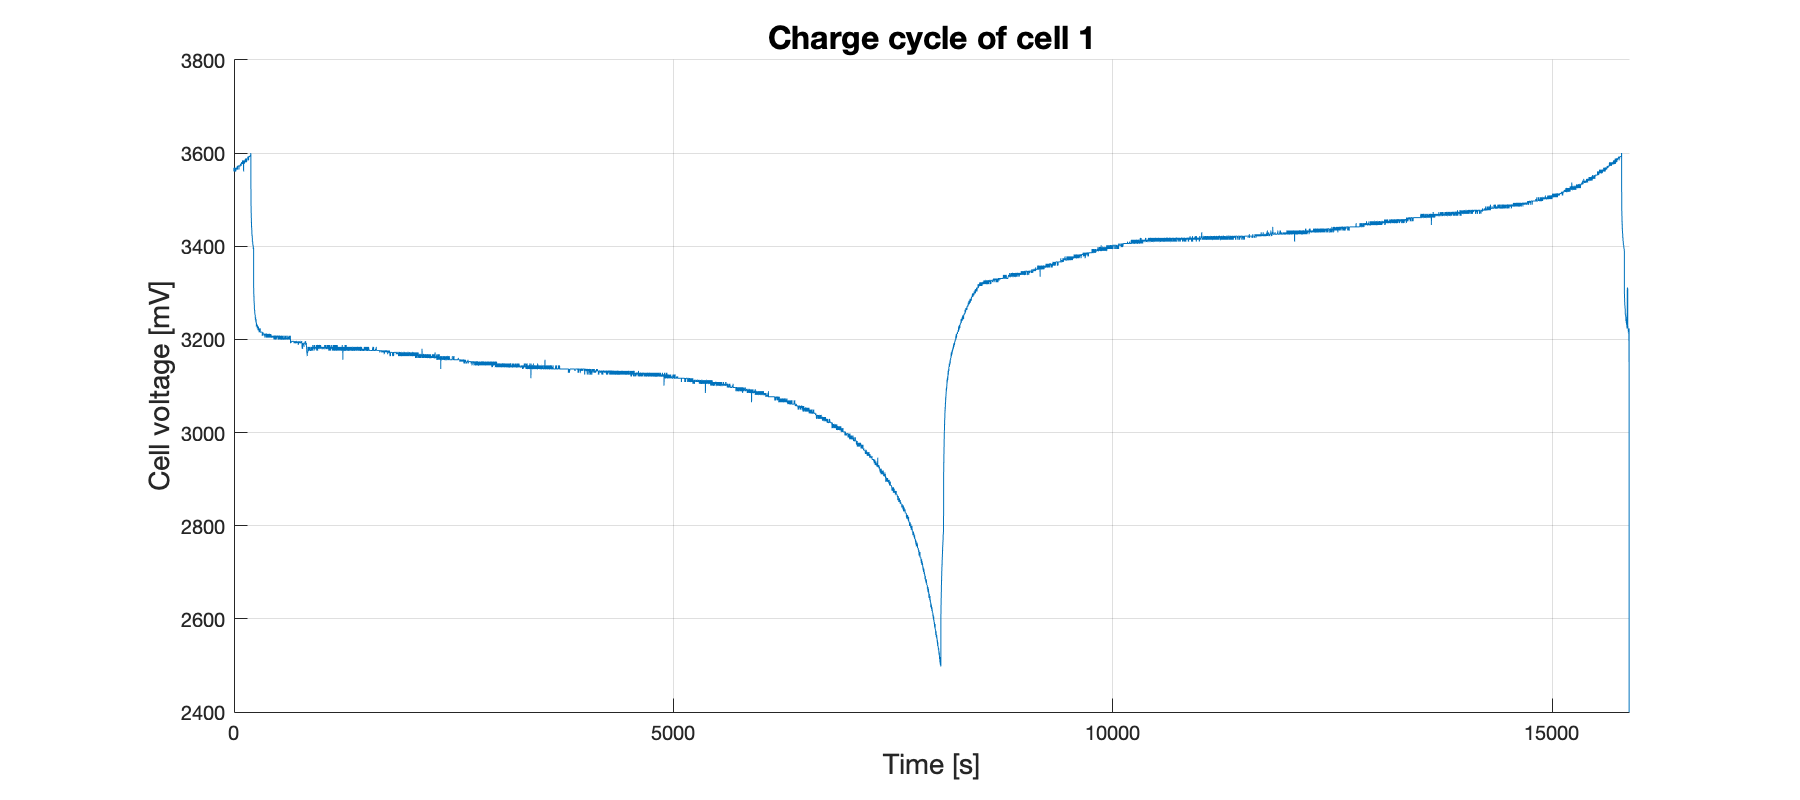
\includegraphics[scale=0.18]{charge_cycle.png}
    \caption{The voltage evolution of cell 1 through a full discharge/charge cycle.}
    \label{fig:charge_cycle}
    \end{figure}

Note the following important points on the graph. At 200 s the cell is done charging and
enters an idle state for 30 s after which it starts discharging. At ~8000 s the cell is fully
discharges and enters an idle state for 30s after which it starts charging. Finally, at 18800 s the cell is once 
again fully charged and the charge cycle is completed.

The provided charging algorithm also logs the current into the cell.
By integrating said current for a full charge or discharge section
we can determine the cell capacity in mAh. The results of this analysis is 
presented in the table below:

\begin{center}
    \begin{tabular}{||c| c c c c c||} 
    \hline
   Cell Number& 1 & 2 & 3 & 4 & 5 \\ [0.5ex] 
    \hline
    Capacity (mAh) & 542.7	& 526.1	& 519.5	& 530.1	& 543.7\\ [1ex] 
    \hline
   \end{tabular}
   \end{center}


As expected all cells have a capacity somewhere around 500 mAh. However, some cells
are have a higher capacity than others which may have implications for the performance
of certain battery cell configurations.

\textbf{\chapter{PV panels}} 
\newline
\newline
The provided PV panels are rated for a maximum power of 1.15 W at a voltage 
of 5.0 V and current 230 mA. Away from the maximum power point the performance of 
the panels can be determined from their I-V curves. To find the I-V curves each 
panel was connected to the B-inputs of the SMPS operating in non-synchronous boost.
They were then lit by the lamp and the duty cycle of the SMPS was varied while measurements 
of panel current and voltage were taken. After processing the resulting data
is plotted in Figure~\ref{fig:IV_curve}.

 \begin{figure}[H]
    \centering
    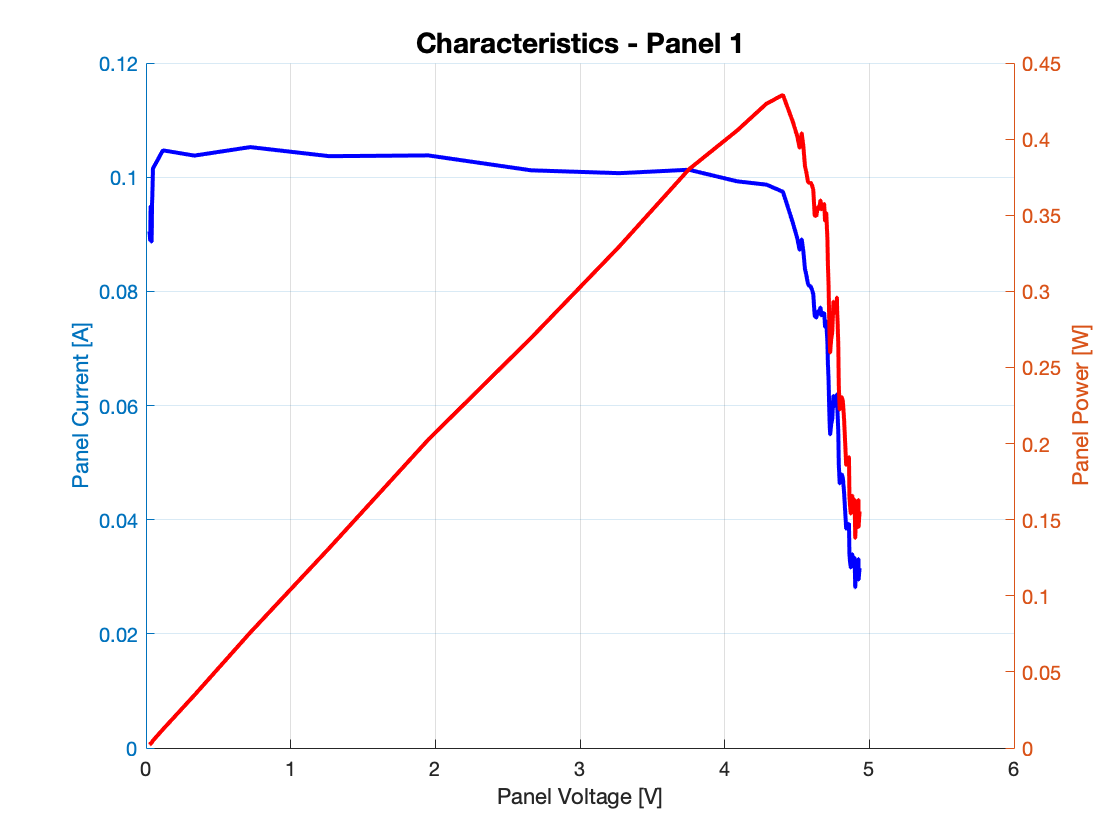
\includegraphics[scale=0.18]{Panel1.png}
    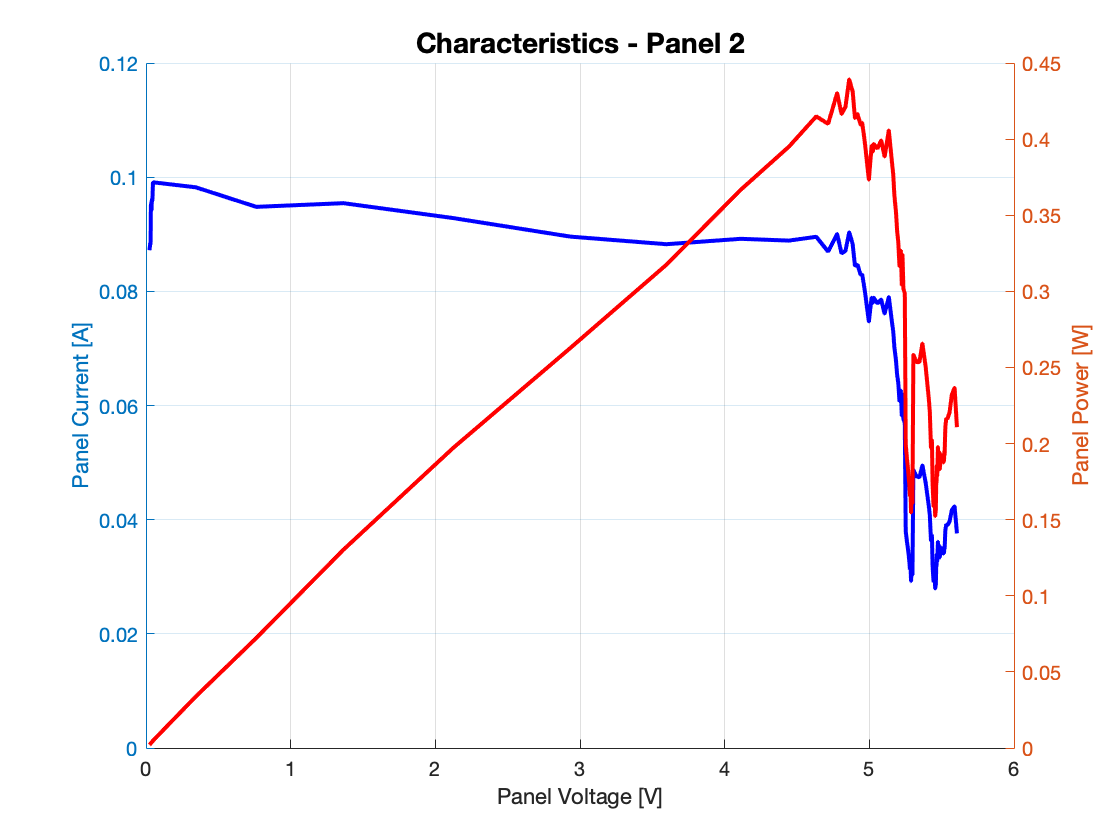
\includegraphics[scale=0.18]{Panel2.png}
    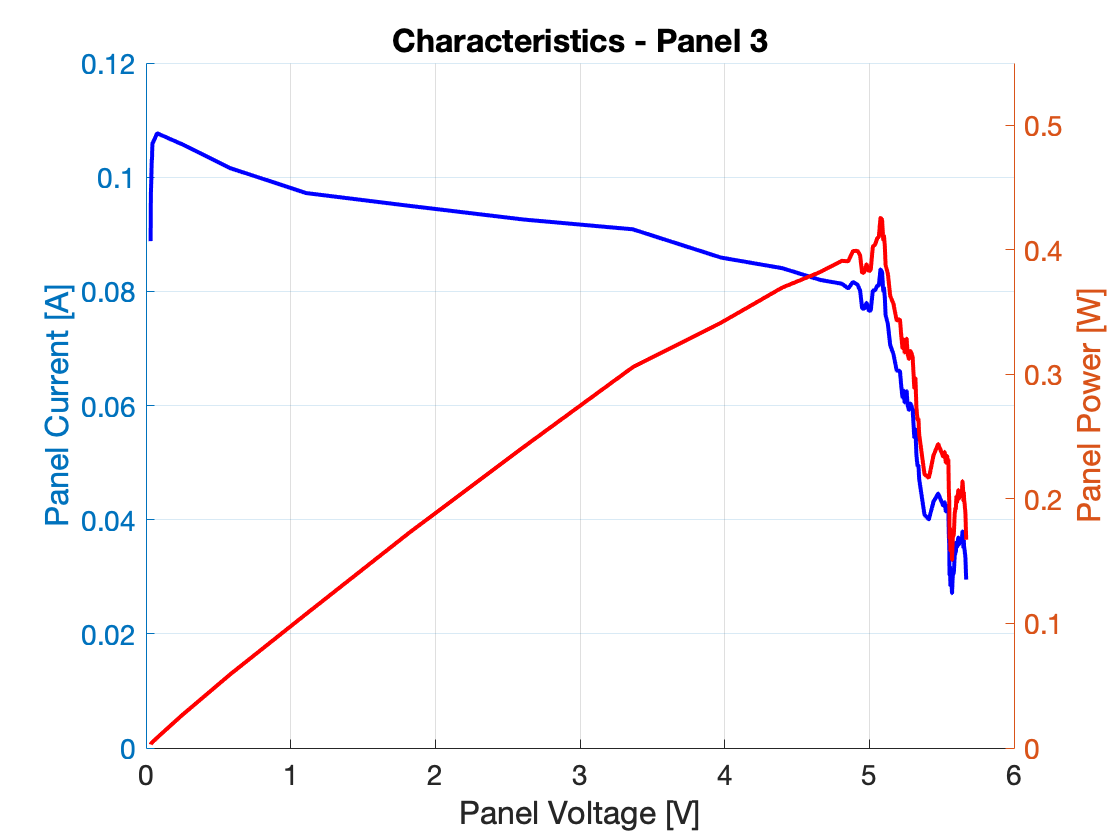
\includegraphics[scale=0.18]{Panel3.png}
    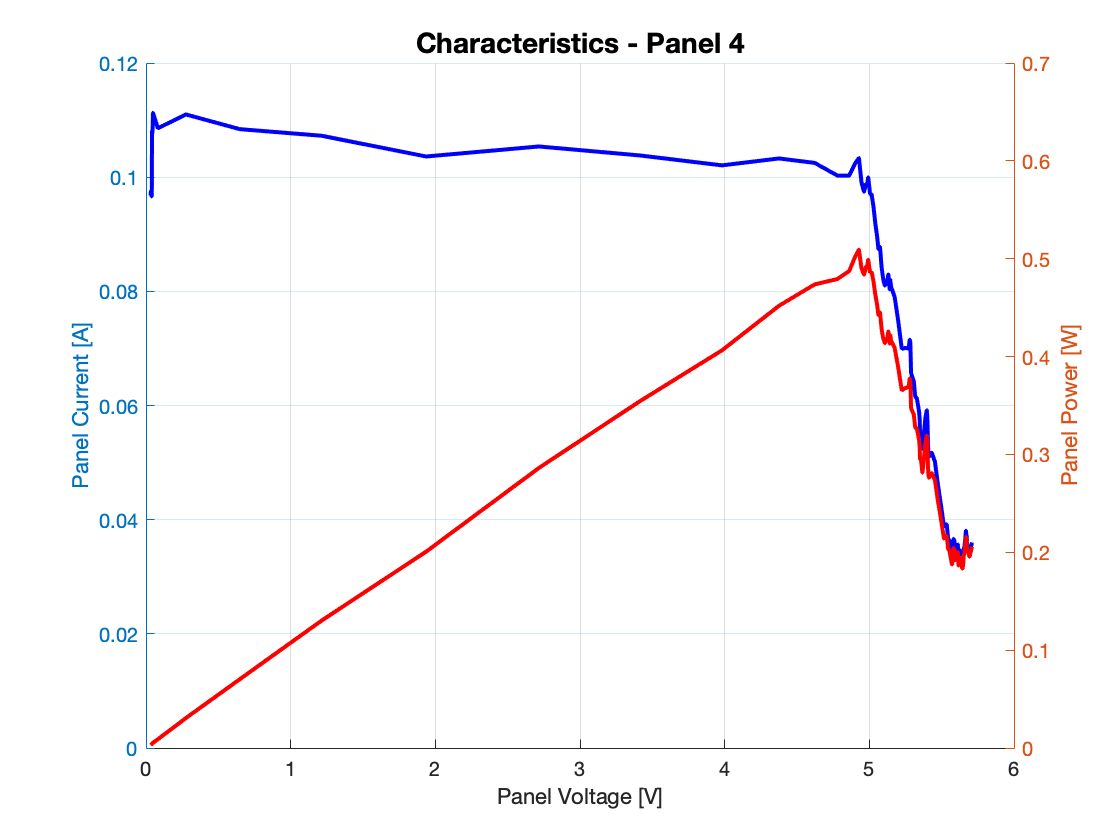
\includegraphics[scale=0.18]{Panel4.png}
    \caption{I-V curves for the PV panels.}
    \label{fig:IV_curve}
    \end{figure}

Though the data is noisy, it is clear that all panels exhibit the standard 
I-V characteristics of a PV cell. That is, they behave as non-ideal current 
sources with a nearly constant current at low voltages and a rapid current 
reduction at high voltages\cite{green}. Moreover, we see that the provided lamp activates 
the panels poorly as the peak power for each of the panels is only ~0.5 W.

\textbf{\chapter{SMPS}} 
\newline
\begin{wrapfigure}[16]{r}[0pt]{0.5\textwidth}
    \begin{center}
      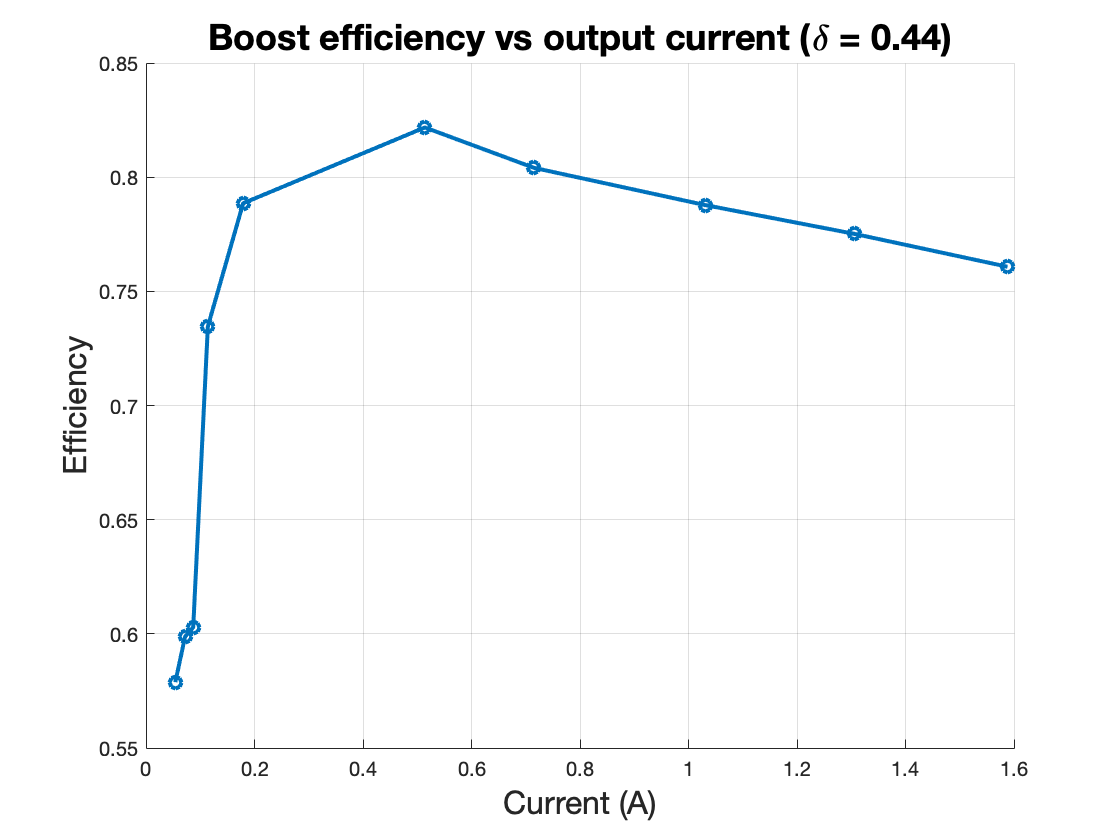
\includegraphics[width=0.48\textwidth]{Boost_efficiency_wduty.png}
    \vspace{0pt}
    \end{center}
    \caption{SMPS efficiency versus output current with input voltage 5V [reference to logbook]}
    \label{fig:efficiency}
  \end{wrapfigure}
The provided SMPS is rated for 10 W throughput with a maximum boost output voltage of 35 V 
and maximum output current of 10 A\cite{SMPS_lab}. All these ratings are far higher 
than needed and neither is expected to impose limitations on the design of the energy module. 

The many characteristics of the SMPS have been thoroughly examined in 
2nd year labs. However, for the energy submodule the most important characteristics 
will be the SMPS efficiency during non-synchronous boost operation. A graph of 
efficiency versus output current is shown in Figure~\ref{fig:efficiency}.


\subsubsection{Battery Configuration}
When designing the battery pack there are two principal choices that need to be made. 
Firstly, how many battery cells should the battery pack consist of and, secondly, 
in what manner should these cells be connected? 

The optimal number of cells is in large part set by the energy 
and power needs of other submodules. During testing the total power 
draw of the rover was found to be about 2 W. Each battery cell has a 
nominal voltage of 3.2 V and a maximum peak discharge current of 1 A 
[battery datasheet], giving a maximum power draw of 3.2 W per cell. 
Thus, to meet the power requirements of the rover it is enough to use only 
one cell. However, each cell can only store about \(3.2 \unit{V} * 0.5 \unit{A} * 3600 \unit{s} \approx 5760 \unit{J} \), 
which would only power the rover for 48 minutes. It is desirable to have 
the rover be operational for as many hours as possible each day. 
Assuming that 12 hours a day are completely without sunlight it is clear 
that the rover cannot work through the night even if all 5 available 
battery cells were used. To give the rover the most operational hours we 
would then want to use all 5 battery cells. However, connecting 5 battery 
boards to the Arduino would use at least 11 of the 12 free Arduino pins, 
leaving only one pin for all other purposes. As such it might be wise to use 
less cells. To accommodate other circuit functions, only 4 cells will therefore be used.

Now consider the PV array. Each PV panel is rated for 1.15 W, meaning 
that the array as a whole should produce 4.6 W. As shown in Figure~\ref{fig:efficiency} the 
peak efficiency of the SMPS in boost mode is about 80\% giving a maximum 
usable power of \(0.8 * 4.6 \unit{W} \approx 3.7 \unit{W} \). Assuming 12 hours of sunlight in a day, 
this means that the PV arra y will produce less energy each day than the rover 
uses in 24 hours. It is therefore of high priority to capture as much of the 
solar power as possible. The battery cells have a standard charging current of 
250 mA \cite{batteryDatasheet}. The power needed to charge the at this current is 
shown in the table below:

\begin{center}
    \begin{tabular}{||c| c c c c c||} 
    \hline
    Number of cells& 1 & 2 & 3 & 4 & 5 \\ [0.5ex] 
    \hline
    Nominal charging power (W) & 0.8 & 1.6 & 2.4 & 3.2 & 4.0\\ [1ex] 
    \hline
    Peak charging power (W) & 0.9 & 1.8 & 2.7 & 3.6 & 4.5 \\ [1ex] 
    \hline
   \end{tabular}
   \end{center}


A 4 cell battery pack is the largest battery pack which has a power 
requirement of less than 3.7 W at standard charging current and little 
power goes unused. Adding to this that the rover has most operational 
hours with 4 cells, using 4 cells is the clear choice. Note that the 
cells used are number 1, 2, 4 and 5 as these were found to have the 
highest capacity.

There are several ways to connect the 4 cells into a power pack, 
however the design brief advised against mixing parallel and series 
connections\cite{energyBrief}. As such only fully series and parallel 
battery packs will be considered. 

A series battery pack has some obvious disadvantages compared to 
a parallel battery pack. In section 2.5.1 it was shown that all the 
battery cells have different capacities. In a parallel battery pack 
this is not a big problem, as it is possible to draw different currents 
from each cell and thereby use the full capacity of each cell. For a 
series battery pack however, the total battery capacity will be limited 
by the cell with the lowest capacity. As such, a series battery pack 
is able to store less usable energy than an equivalent parallel battery 
pack. Moreover, to check the OCV of each cell they need to be switched 
out of circuit using the battery board relay. For a series battery pack 
this leads to an open circuit and any charging/discharging of the battery 
must halt while the voltage is measured. For a parallel battery pack on the 
other hand, switching the relay of a cell only takes that one cell out of 
circuit and it is possible to charge/discharge the battery pack while 
taking voltage measurements. Being able to switch single cells out of 
circuit can also enables switching faulty cells out of circuit, meaning 
that one cell failing would not mean that the battery pack as a whole fails. 
Finally, a parallel battery pack is self-balancing and energy automatically
flows between cells when necessary\cite{batteryBalancing}. Series cells on the 
other hand need to be balanced by switching on and off balancing resistor. 
This not only is more complex, but leads to power being lost in the balancing
resistors.

There is however one major weakness to a parallel battery pack: 
it is very hard to track the current going into individual cells. For 
safe operation it is necessary to prevent over-current into each individual 
cell. However, the current sensor on the SMPS can only measure the current 
flowing into the battery pack as a whole. Each battery cell is only rated 
for a rapid charging current of 500 mA\cite{batteryDatasheet},  and seeing 
as there is no way to know how the current splits into each of the cells 
one must operate one must operate with the assumption that all the current 
can flow into a single cell. As such, no more than 500 mA can be allowed 
to flow into the battery pack as a whole. At this current the nominal 
charge power is only \(3.2 \unit{V} * 0.5 \unit{A} = 1.6 \unit{W} \)
 meaning charging will be slow and it is only possible to use less than half of the available solar power. 
This is such a large drawback of using a parallel battery pack, that 
despite all the previously stated disadvantages of a series battery pack, 
a series battery pack has been deemed the best option.

\subsubsection{PV Array Configuration}

To facilitate the highest power output all the four provided PV panels will be used.
 There are four different ways in which the four panels can feasibly be connected. 
 The different arrangements are shown in figure~\ref{fig:arrayConfigurations}.

 \begin{figure}[H]
    \centering
    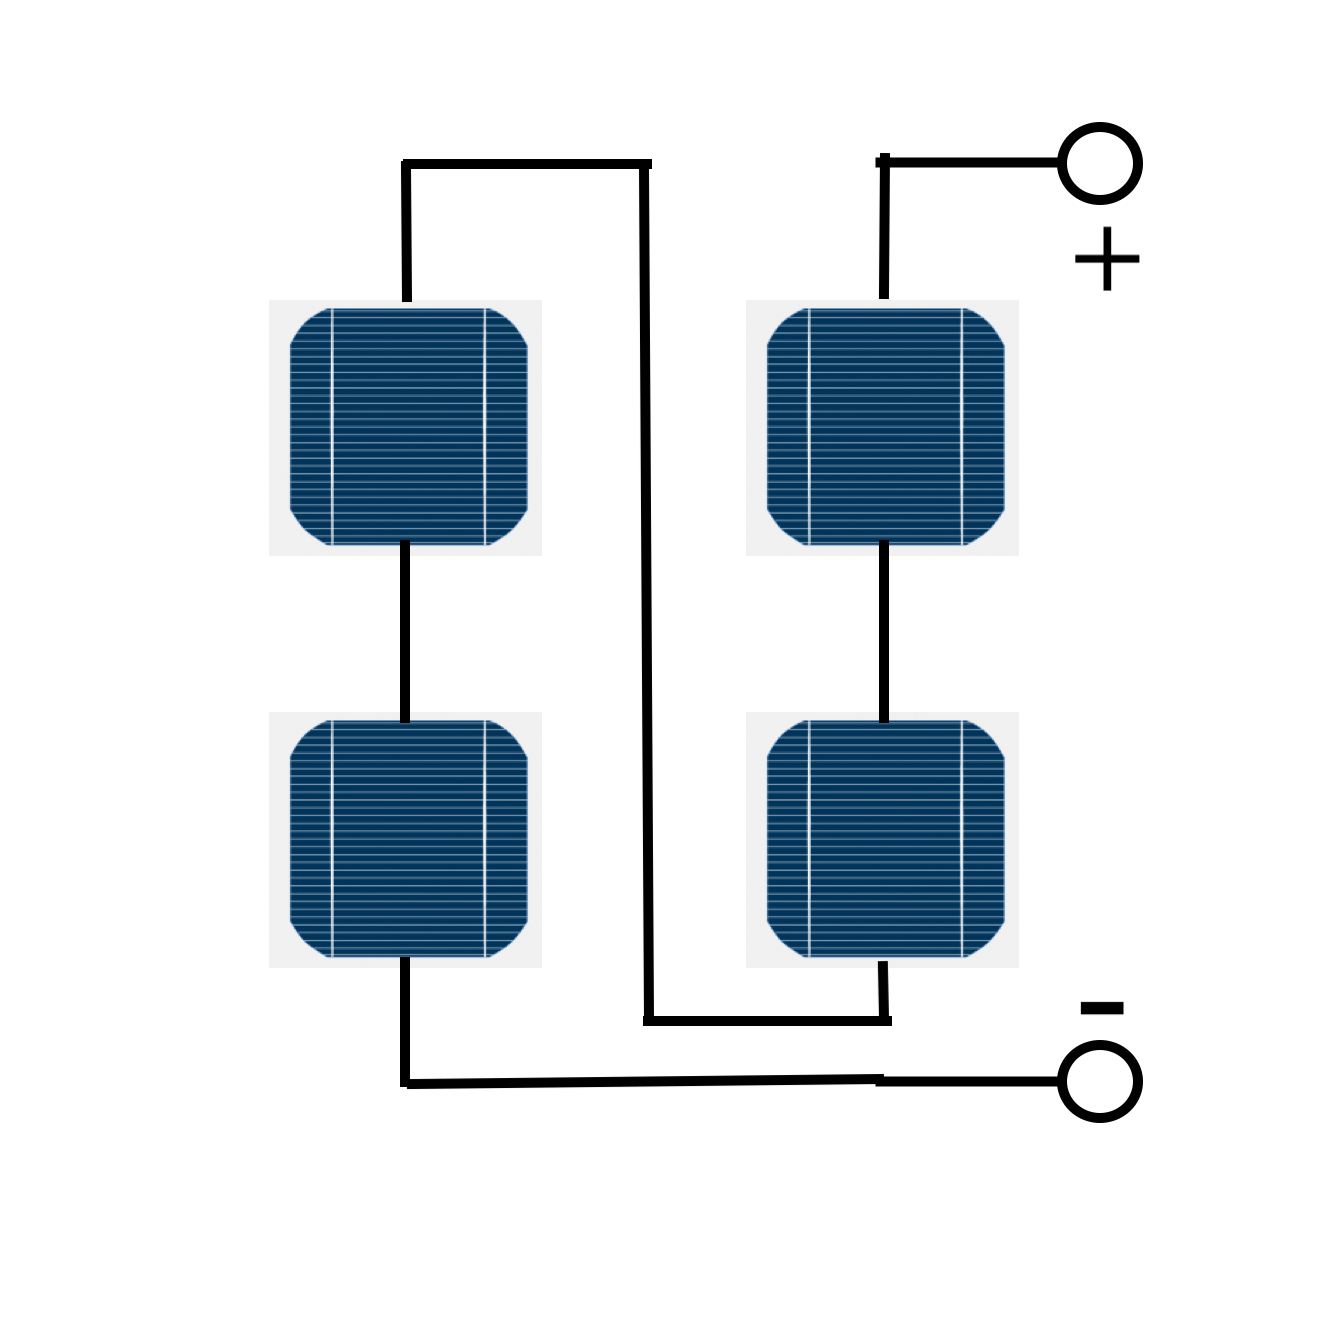
\includegraphics[scale=0.10]{Series(S)}
    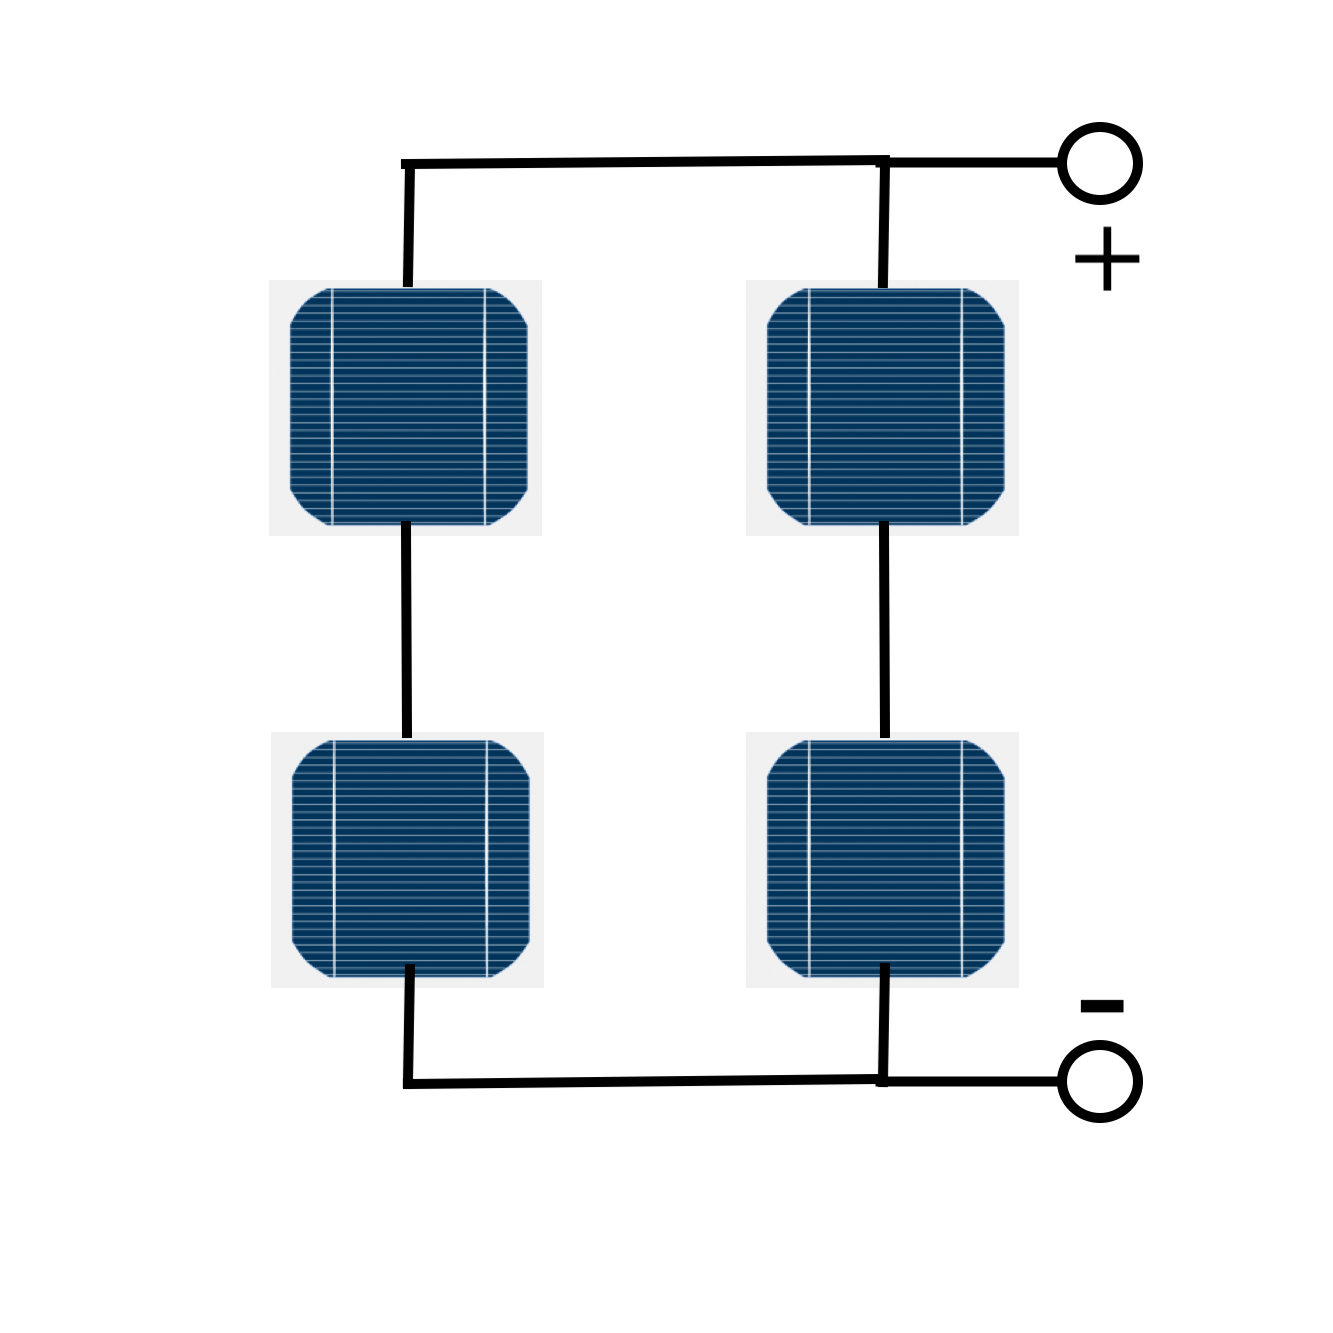
\includegraphics[scale=0.10]{Series-parallel(SP)}
    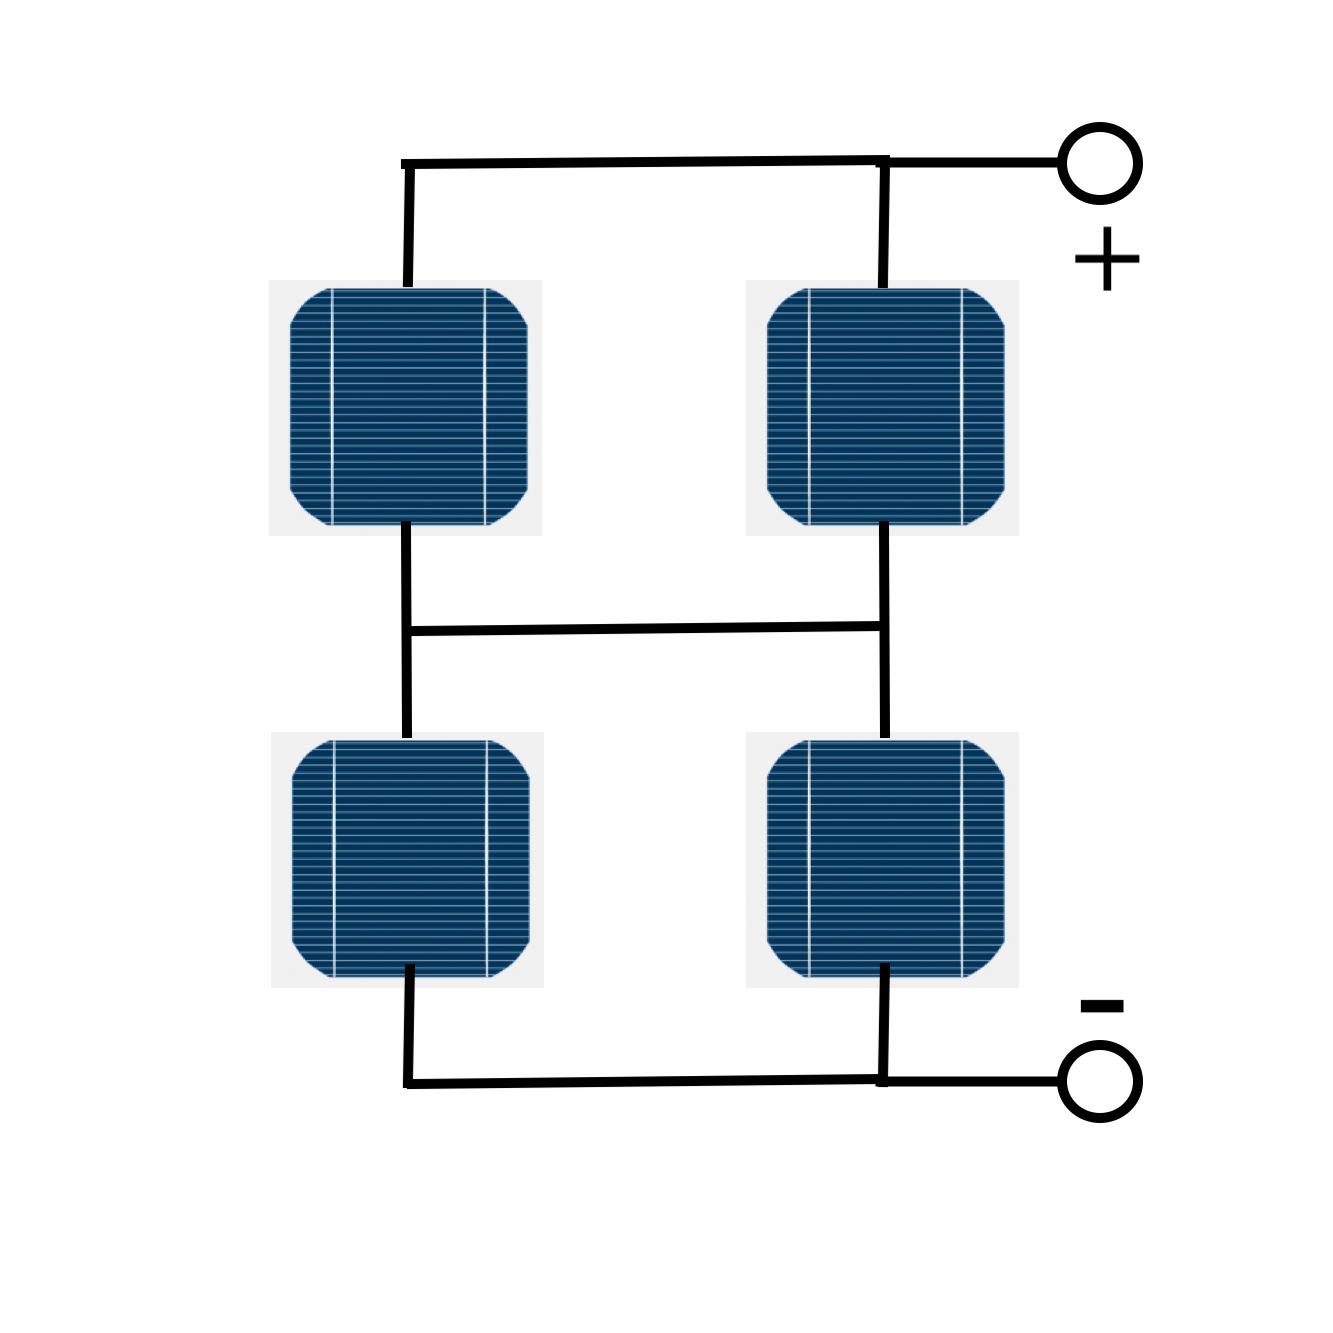
\includegraphics[scale=0.10]{Total-cross-tied(TCT)}
    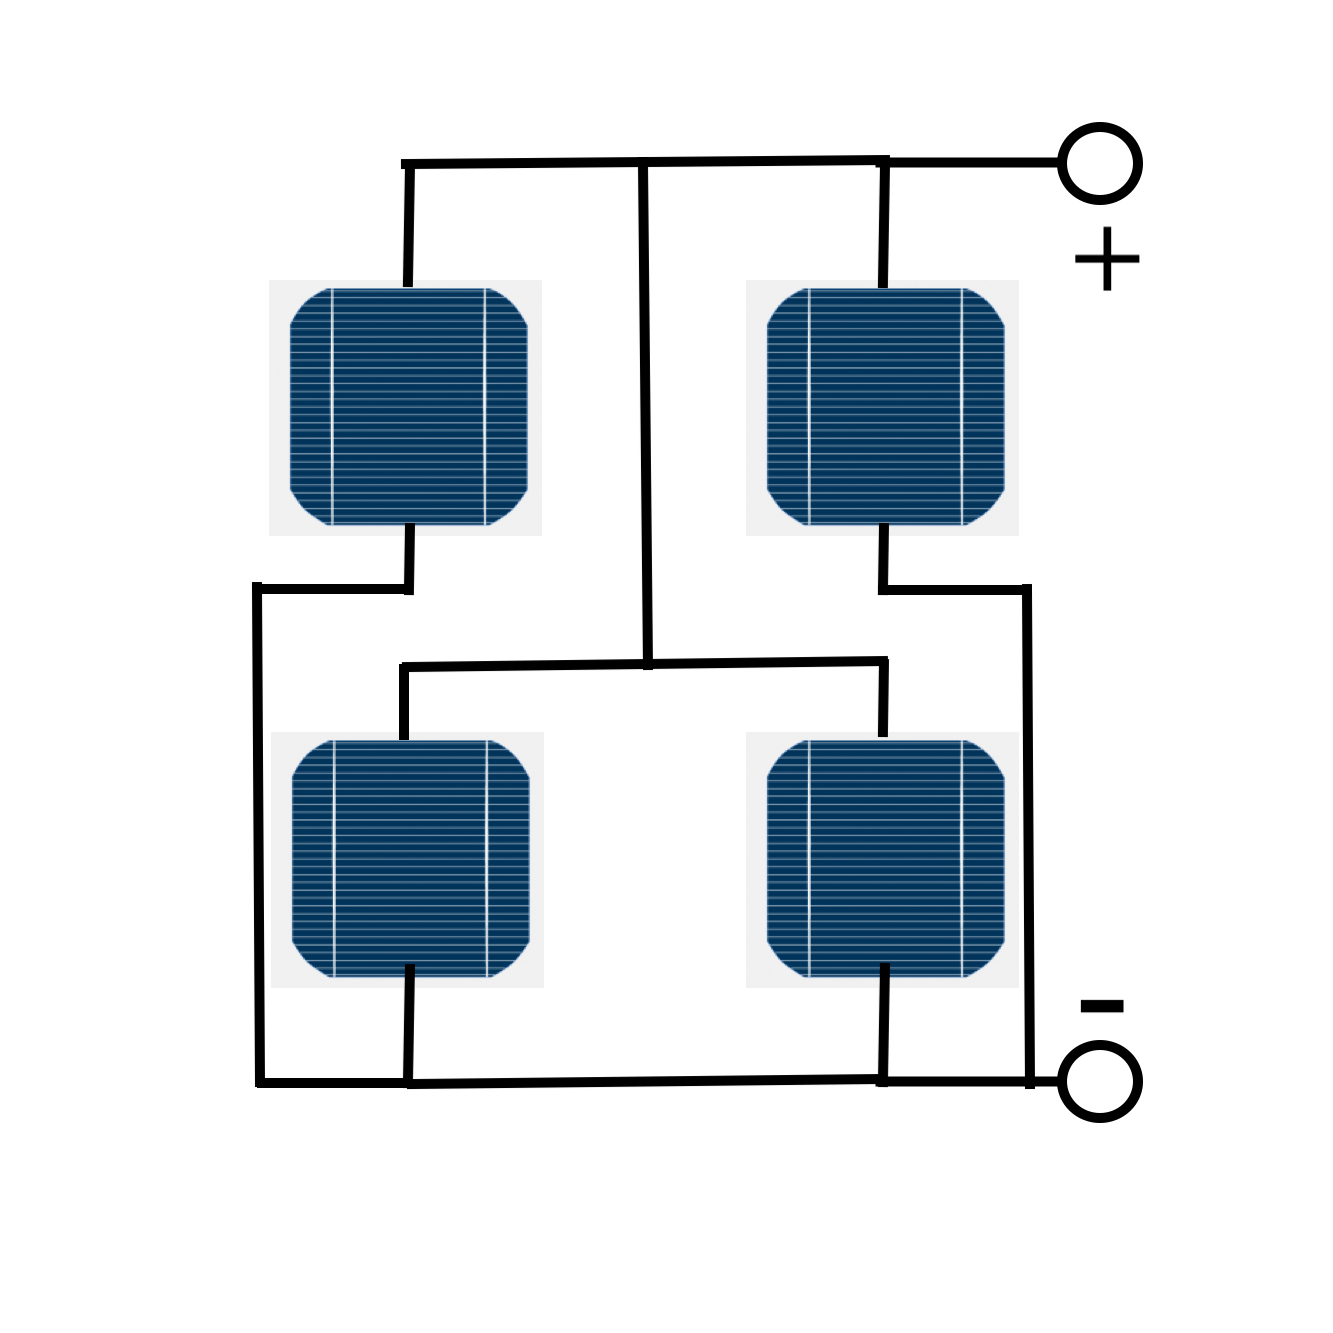
\includegraphics[scale=0.10]{Parallel(P)}
    \caption{From left to right: Series (S), Series-Parallel (SP), Total-Cross-Tied (TCT), Parallel (P)}
    \vspace{-10pt}
    \label{fig:arrayConfigurations}
\end{figure}


However, considering the array voltages it is clear that the only viable arrangement 
is the purely parallel connection. Consider first a pure series connection. In 
section 2.5.1 each PV panel was found to have a max voltage of around 5.5 V. 
The series connection will therefore have a total voltage of about 20+ V. 
The nominal voltage of the series battery pack is \(4 * 3.2 \unit{V} = 12.8 \unit{V} \). As the array voltage is higher than the battery voltage, the SMPS must 
be used in the buck configuration. However, the maximum buck input voltage 
is only 7 V\cite{PMOS} and therefore a series connected PV array 
cannot be used. Similarly for the Series-Parallel and Total-Cross-Tied 
arrangements the maximum array voltage will be about 11 V. However, 
as will be discussed in section 2.5.6 the battery pack voltage will 
swing between 10 V and 14.4 V in a charge cycle. The problem is that 
the 11 V array voltage is lower than the highest battery voltage, but
 higher than the lowest battery pack voltage. For the array configuration
to charge the battery pack it would then be necessary to have a power
converter which can both step up and down voltage. Depending on how the 
SMPS is configured it can either function in buck or boost mode, both not 
both at the same time. Thus it is not possible to use either the Series-Parallel
or Total-Cross-Tied configuration. This leaves a purely parallel battery 
pack as the only viable option, which is why it has been chosen. 


\subsubsection{SMPS Configuration}
As the voltage of the battery pack is higher than the voltage of the series 
connected battery cells, the voltage of the solar panels must be stepped up 
when used for charging. This means that the SMPS must be operated in boost 
mode with the solar panels on port B and battery on port A. Moreover, as the 
SMPS has a max output voltage of 7 V in synchronous boost operation\cite{powerLogbook}, 
it must be operated in non-synchronous mode.

\subsubsection{Maximum Power Point Tracking}
Power provided by PV panels often has to be condition before use. Commonly this 
is done through the use of a two-stage power converter. The first stage of the power
converter does maximum power point tracking to ensure the panels provide as 
much power as possible. The second stage ensures that the power is exported at the
required voltage or current\cite{green}. As the energy submodule only has
access to a single SMPS device it is not possible to implement such a two stage
power converter. Meaning that at any time it will only be possible to either operate 
at the maximum power point or have the power be outputted at the correct current/voltage.
This is however not a problem as the goal of the PV panels is not to output the 
maximum amount of power, but simply to provide the power demanded by the charging algorithm. 
As will be shown in later sections, during charging it is desirable to draw a set
current from the SMPS output. Even if the PV panels could produce more power i.e.
provide a higher current than what is being drawn, it is not desireable to increase 
the output current. As such, the system does not need conventional MPPT. However,
as is discussed below, if the PV panels cannot provide the demanded power some sort 
of power tracking must be implemented. 

\begin{wrapfigure}[18]{r}[0pt]{0.5\textwidth}
    \begin{center}
      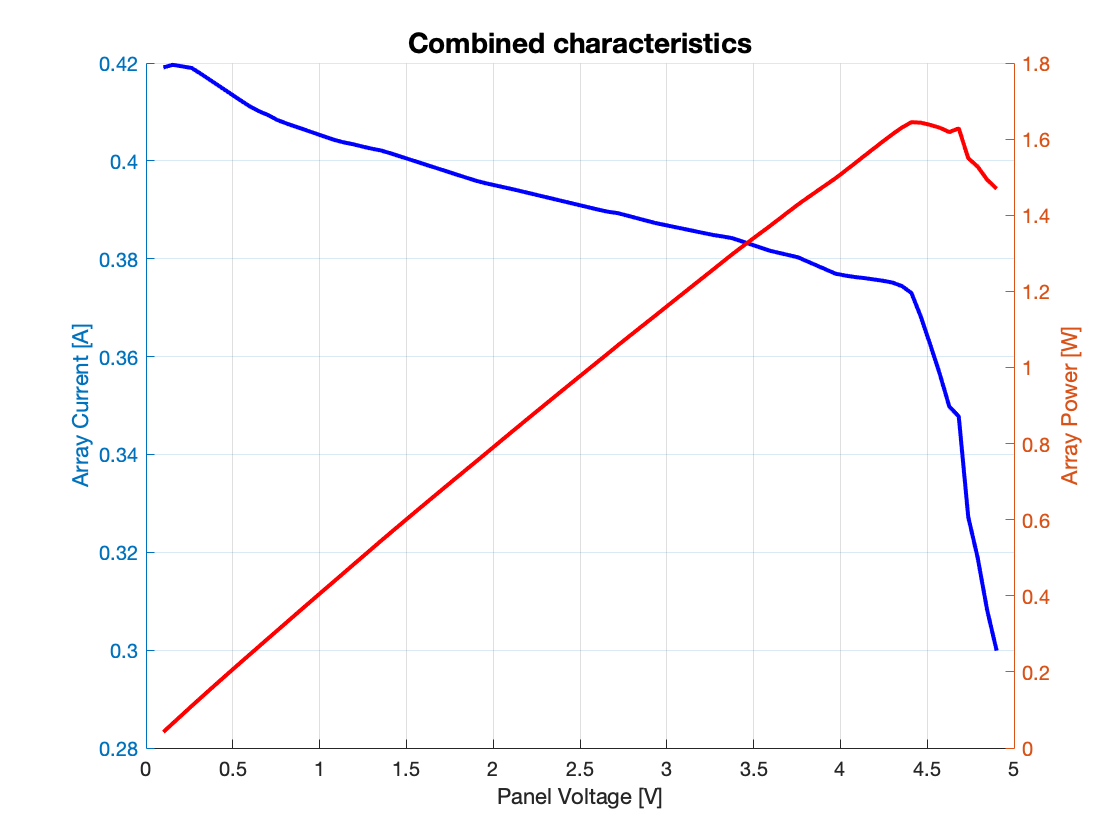
\includegraphics[width=0.48\textwidth]{Combined.png}
    \vspace{-15pt}
    \end{center}
    \caption{IV-curve (blue) and power curve (red) of the parallel configured PV array lit by lamp}
    \label{fig:parallelArray}
\end{wrapfigure}

Consider an SMPS being used to charge a battery pack at a set current. 
If the actual current on the output is lower than the setpoint, one would attempt
to increase the output current by increasing the output voltage. For an SMPS this
is achieved by increasing the duty cycle. Similarly, if the output current is too
high one would attempt to lower the output current by lowering the duty cycle. From 
these considerations we see that increasing and decreasing the duty cycle is 
associated with higher and lower output power respectively. Now compare this with
the IV and power characteristics of the parallel PV array shown in 
Figure ~\ref{fig:parallelArray}. For an SMPS, increasing the duty cycle 
will lower the input resistance, causing the input current to increase. As increasing
the duty cycle increases the output power so too must increased input current lead to
increased input power for an equilibrium to exist. However, increased input current
only gives increased output current if the PV panels are operating in the region to the right of the
maximum power point. Thus this is the region one would want the panels to operate in.

To ensure that the PV panels are operating in the correct region, start with a duty
cycle of 0 and increase it until the output current/voltage is at the desired value.
If the desired operating point requires less power than what the PV array can provide,
then an equilibrium should be found as the duty cycle is increased. If however the 
desired operating point requires more power than the PV panels can provide, then no 
equilibrium can exist and the duty cycle will increase to 1 without ever reaching the
desired operating point. Thus, if the duty cycle ever reaches 1 during operation
the charging algorithm must be trying to draw more power from the SMPS than is 
possible. If so, the charging algorithm must be told to operate a lower power point. How this
is implemented is covered in section ....

\subsubsection{State of Charge}
The state of charge (SOC) of a battery is defined as the remaining usable charge 
given as a percentage of the battery’s total charge capacity\cite{DICKINSON2009452}. There are many 
methods for  estimating the SOC of a battery, the most common of which rely on 
measurements of the voltage and/or current of the battery\cite{DANKO2019186}. The perhaps 
simplest SOC estimation method is to measure the open circuit voltage (OCV) 
of the battery and then calculate the SOC using a formula or a lookup table. 
For many types of battery this is a good estimation method. An example is 
lead-acid batteries, for which the OCV varies approximately linearly with the 
SOC. However, as was shown figure ~\ref{fig:efficiency}, this is not the case 
for LiFePO4 batteries. For LiFePO4 cells the voltage is nearly constant for 
a majority of each charge/discharge cycle. Any measurement error or change in 
OCV due to current recently flowing through the battery, would therefore produce large 
SOC estimation errors. This holds true for all SOC methods relying purely on 
voltage measurements and they are therefore not good alternatives. 

An alternative SOC estimation method is Coulomb counting, where the current 
flowing through the battery is integrated to find the net charge that has 
left or entered the battery. Seeing as charge is a conserved quantity nearly 
all charge put into the battery will be available during discharge. As such, 
the SOC will vary nearly perfectly linearly with the integrated current. 
The sources of error for Coulomb counting are mainly the Coulombic efficiency 
of the batteries and current measurement errors. However, using correction 
methods the error can be kept small, on the order of 1-2\%\cite{NG20091506}. Given the 
simplicity of the estimation method, this is a very small error. Other 
estimation methods, such as Kalman filters and neural networks, are claimed 
to give higher estimation accuracies\cite{DANKO2019186}. However given the already high 
accuracy of Coulomb counting the improvement is marginal. Moreover, they 
are far more complex both computationally and in implementation. As such, 
Coulomb counting was deemed the best option for SOC estimation.

SOC is a measure of charge and not energy. It is necessary to estimate 
the range of the rover. The obvious way of doing this is to track the 
power consumption and speed of the rover. Dividing the energy left in 
the batteries by the power and multiplying by the speed gives an estimate 
of the range under the current operating conditions. The problem however, 
is that the SOC only gives the usable current and not the usable energy 
left in the battery. As the SOC of the battery decreases, so too does it 
voltage, meaning that at lower states of charge each mAh will provide less 
energy than at higher states of charge. To account for this, during discharging 
the BMS logs the energy output of the battery alongside the SOC. From this data 
it is possible to create a lookup table which relates the current SOC to how 
much energy it is still possible to draw from the battery. This is the method 
which will be used to find the energy left in the battery. 

\subsubsection{State of Health}
The state of health of a battery is a measure of its current condition and 
performance compared to when it was new\cite{mpower}. Indicators of a battery’s state 
of health include battery charge capacity, energy capacity, cell voltage 
balance, and the number of completed charge/discharge cycles\cite{https://doi.org/10.1002/er.3598}. All these 
indicators are tracked during operation and stored on the SD-card as to 
retain data when the Arduino is not being powered. Over the course of its 
lifetime the SOH of a battery will naturally degrade. However, through SOH 
maintenance the degradation can be slowed significantly. Most importantly 
for a series battery pack is to keep the battery cells balanced, as 
unbalanced battery cells lead to lower capacity and faster cell degradation\cite{texas}. 

To facilitate balancing, each of the provided battery boards have mounted 
resistors which through a MOSFET can be connected to the battery cell. 
Connecting a cell to the resistors on the battery board will lead to a 
small extra current flowing out of the cell, slowly discharging it. 
During operation one must decide when to switch said resistors on and 
off to keep the cells balanced. Usually, balancing is only done towards 
the end of a charge cycle\cite{texas}. There are several reasons for this. Firstly, 
passive balancing requires energy to be expended and will therefore reduce 
the total amount of usable energy in a battery if done during discharging. 
Secondly, differences in impedance and charge curves between cells might 
make it look as though a cell is charged more than others, but the voltage 
difference might disappear naturally as the battery is charged more or as 
charge current is reduced towards the end of a charge cycle. As such, the 
implemented charging algorithm only does balancing during the constant 
voltage part of charging. The balancing is done using the code shown in 
Figure~\ref{fig:balancingCode}. During CV charging it is desirable that all cells have a voltage 
of 3600 mV. If any cell has a voltage which is higher than 3600 mV its 
voltage is too high and the dissipative resistors are switched on to lower 
the voltage to the voltage set point. 

\begin{figure}[H]
    \centering
    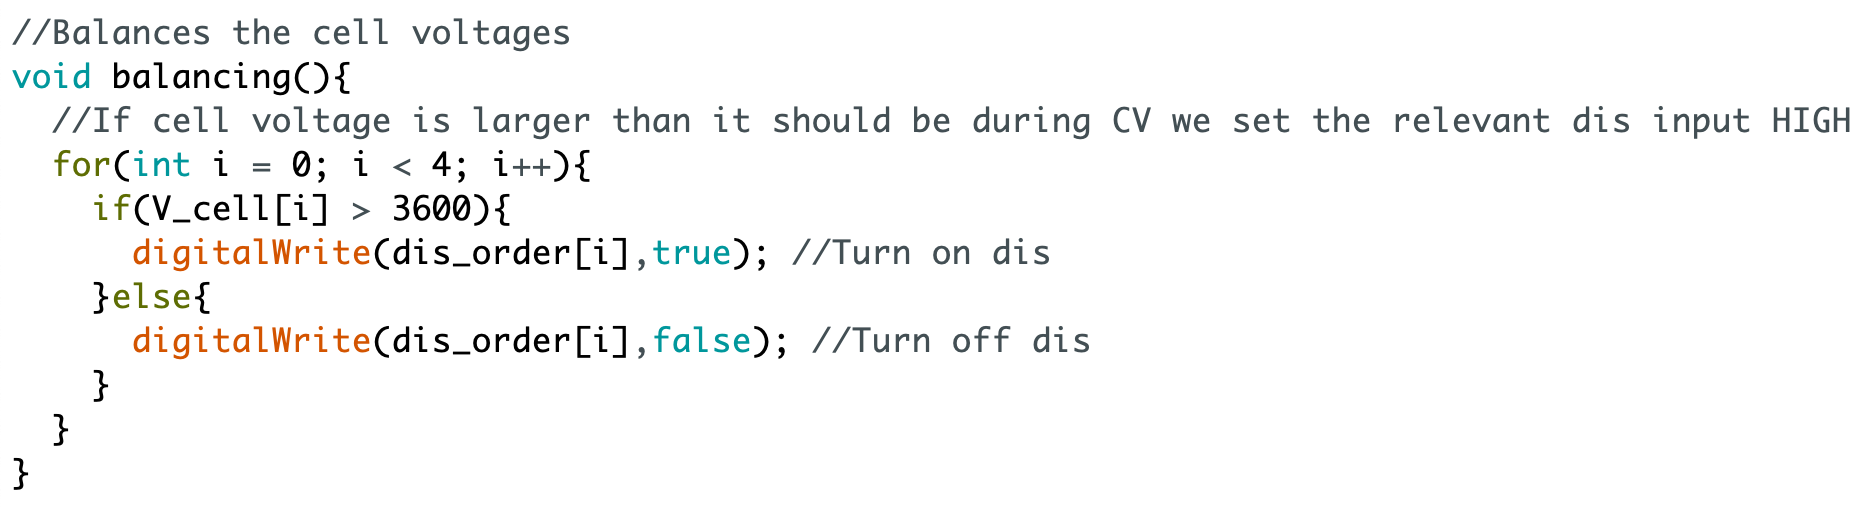
\includegraphics[width = \textwidth]{Balancing_code.png}
    \caption{Function called while charging at high SOC to balance out the voltage of the cells.}
    \vspace{-10pt}
    \label{fig:balancingCode}
\end{figure}

Alongside the constant voltage charging algorithm this code was extremely 
successful at balancing the cells. The balancing is shown in action in Figure~\ref{fig:balancing}. 
One by one, the cell voltages are brought up to and kept at 3600 mV. Even with 
an initial voltage difference of 200 mV, balancing only takes about 
1000 seconds = 17 minutes. 


\begin{figure}[H]
    \centering
    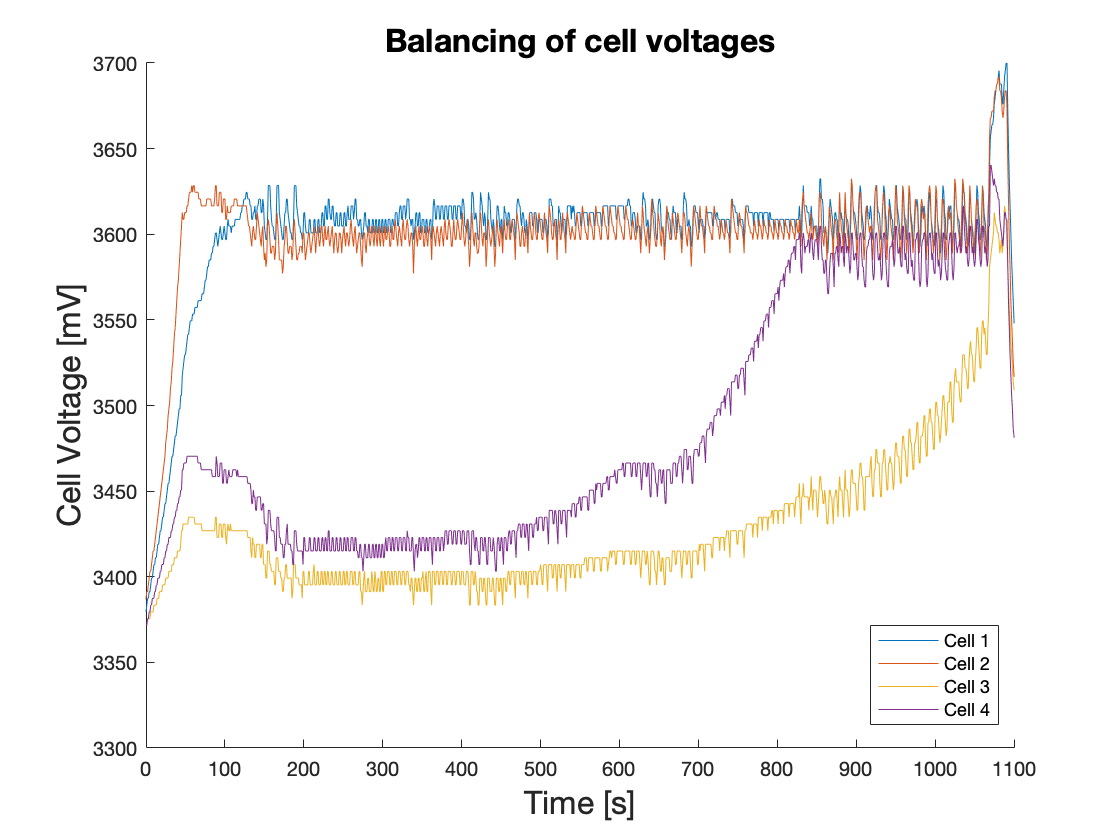
\includegraphics[width=0.48\textwidth]{balancing.png}
    \caption{Cell voltages as they are being balanced, ignore voltage spikes at end as they are not related to the balancing.}
    \label{fig:balancing}
\end{figure}

\subsubsection{Communicating with Other Modules}
Though it is not necessary to fully integrate the energy module with the rest of the rover, other submodules, specifically command, needs access data such as the battery SOH and SOC. For communicating with other modules the Arduino shield has a set of UART ports. However, as group members were not in the same location it was not possible to physically connect the energy module to the rover, which is necessary to use UART. As such, an alternative approach was employed. First the Arduino was connected to a computer via USB. On the computer a Python script was run [8]. At the start the Python script establishes a connection to a server created by running a similar script on the command module [9]. After a connection has been established the Python script starts reading the serial data coming from the Arduino and transmits it using TCP to the command module. Each message coming from the Arduino is in CSV form where the first entry is the message ID, which allows the command script to decode what type of data is being sent. 

What data do we send?
\subsubsection{Physical Integration of the Energy Module}

\subsubsection{Implementation}
Added mosfet as voltage divider by itself gave unreliable results, arduino can draw

\subsubsection{Tracking SOH and SOC during discharging}

\subsubsection{Safety Mechanisms}

\subsubsection{Charging Algorithm}

% End of energy subsection

\subsection{Integration}



\section{Evaluation and Conclusion}

\section{Project Management and Organisation}
%Also had frequent teams meetings and used WhatsApp
As this project was carried out remotely
with contributors located in different countries, 
it was important to have a good framework for communication and management. 

The main tool used for communications and management was Git + GitHub.
As the codebase was incredibly complex, 
involving many different libraries and with each submodule being capable as a
standalone project, it was vital to have a version control system in place. 
Being able to keep a history of commits and changes made to a project was useful,
especially when trying to track down the origin of a bug and what caused it. 

The team also made use of GitHub Issues to track progress and accountability in 
the initial design phase. A thread was opened for each submodule to show what 
the lead for that submodule had been doing and potential avenues of achieving 
their goals. This was beneficial both for the leads to keep track of their 
research, but also allowed other members to contribute to other submodules 
by adding comments and voicing their thoughts. GitHub Issues were also linked 
directly to commits in the codebase to allow for a more in-depth explanation and
reasoning with context for a commit than what is allowed in the commit message 
area. 

Simultaneously, a Gantt chart was maintained to keep track of progress and is 
available for viewing under the maintained GitHub repository linked in the Appendix.

%TODO #7!
\section{Intellectual Property}
\begin{comment}
Could link stuff about how we are using Intel IP in the FPGA, as well as things
like licencing and how some companies make their entire business based on it,
like Arm, hence ethically it is important to maintain standards and rules for IP
through the use of legislation and governmental regulatory authorities. 
\end{comment}
\begin{comment}
A lot of the technologies that we have used in this project is probably covered
by a patent.
\end{comment}


\newpage

\printbibliography[
heading=bibintoc,
title={References}
]


\begin{figure}[H]
\centering

\includegraphics[scale=0.18]{logo.png}
\caption{Sample Figure}
\label{fig:image1}
\end{figure}

Sample Reference\cite{einstein}


\begin{appendices}
\chapter{Some Appendix}
The contents...
\end{appendices}

\end{document}